\documentclass{beamer}
\usepackage{forest}
\usepackage{cgloss4e}
\usepackage{tikz}
\usepackage{gb4e}
\usetheme{Boadilla}
\usetikzlibrary{calc}
\usetikzlibrary{matrix}
\usetikzlibrary{positioning}

\title{Scope without Syntax}
\subtitle{Towards a Game Theoretic Approach}
\author{Luke Smith}
\date{September 27, 2017}
\institute{Committee: Robert, MPP, TgB}
\usetikzlibrary{shapes.geometric, arrows}

\tikzset{Above/.style={midway,above,font=\scriptsize,text width=1.5cm,align=center,},Below/.style={midway,below,font=\scriptsize,text width=1.5cm,align=center}}
\tikzstyle{box} = [rectangle, centered, draw=black,minimum width=3cm, minimum height=1cm]
\tikzstyle{arrow} = [thick,->,>=stealth]

\tikzset{centered/.style=}


\begin{document}

\resetcounteronoverlays{exx}

\begin{frame}
\titlepage
\end{frame}

\section{Background}

\begin{frame}
\frametitle{Quantifiers}\pause
\begin{itemize}
\item Languages have what are called \emph{quantifiers}, which are words which delineate particular quantities of nouns that they modify.\pause
\begin{itemize}
\item \textbf{Universal quantifiers} -- all, each, every ($\forall$)\pause
\item \textbf{Existential quantifiers} -- a, one, some ($\exists$)\pause
\item \textbf{Negation} -- not, no ($\neg$)\pause
\item Many others -- numerals, much, many, few, etc.\pause
\end{itemize}

\item For the purposes of sentence interpretation, quantifiers are quite a puzzle. Especially when there are multiple quantifiers in a sentence, a sentence may become ambiguous.
\end{itemize}

\end{frame}

\begin{frame}
\frametitle{Scope Ambiguity}\pause
\begin{exe}
\ex Everyone loves someone.
\end{exe}\pause
\begin{itemize}
\item This sentence has two quantifiers, a universal ($\forall$) `every' and an existential ($\exists$) `some.'\pause
\item This sentence has two different interpretations:\pause
\begin{itemize}
\item For each person, there exists some other person  they love.\pause
\item There exists one particular person who everyone loves.\pause
\end{itemize}
\item In the first possible reading, we say that the $\forall$ takes `wide scope' over the $\exists$, which is said to have `narrow scope.'\pause

\item In the second, we say that the $\exists$ takes wide scope over the $\forall$.
\end{itemize}
\end{frame}

\section{Scope in the Field}

\begin{frame}
\frametitle{Traditional View}\pause
\begin{itemize}
\item Scope was traditionally dealt with in terms of `movement' and `logical form.' An ambiguous sentence had to go through some kind of post-syntactic change to yield an unambiguous representation in the mind.\pause
\item Different languages were discovered to have different availabilities of scope ambiguity. This was dealt with with formal and syntactic parameters.\pause
\item Over wide enough data sets, few generalizations were robust.\pause
\item Scope ambiguity is difficult to account for because it is:\pause
\begin{itemize}
\item Highly context sensitive (Chomsky's aphasia)\pause
\item Sensitive to linear order 
\end{itemize}
\end{itemize}
\end{frame}

\begin{frame}
\frametitle{Game Theoretic Scope}\pause
\begin{itemize}
\item \textbf{My statement:} Scope ambiguity is totally paralinguistic. Scope ambiguities fall out from listeners' evaluation of the intentions of the speaker.\pause
\item We don't need ``syntax'', we don't need ``logical form'', we don't need any linguistic machinery whatsoever.\pause
\item This can partially be modeled in Game Theory, seeing that speakers are mutually evaluating the others' behavior and choosing how to word or interpret sentences based on that.\pause
\item This can allow us to formally analyze an apparent ``functional'' alternation.
\end{itemize}
\end{frame}

\begin{frame}
	\frametitle{Game Theory Abridged}

	\begin{itemize}
		\item Theoretical framework for analyzing decision-making, conflict and cooperation.\pause
		\item The gist:\pause
			\begin{itemize}
				\item Have a set number of players.\pause
				\item Each player has a set of possible behaviors ``strategies''.\pause
				\item Players are awarded payoffs based on the strategies taken by each player.
			\end{itemize}
	\end{itemize}
\end{frame}

\begin{frame}
\frametitle{Precedents in Linguistics}\pause
\begin{itemize}
\item Game Theory has been similarly employed in linguistics, particularly semantics to deal with implicatures.\pause
\begin{exe}
\ex Billy ate most of the chocolates.
\end{exe}\pause
\item Sentences like this in actual language are inferred to mean that Billy ate most \emph{but not all chocolates}, although the sentence is logically still true if he did.\pause
\item However speakers \emph{assume} Billy didn't eat \emph{all} the chocolates because if that were true, a speaker probably would've said so.\pause
\item Normal human:\pause
	\begin{itemize}
		\item ``If he wanted to say `Billy ate all the chocolates', he would've said just that!''
	\end{itemize}
\end{itemize}
\end{frame}


	\begin{frame}
	\frametitle{Our Quantifier Scope Game}

\begin{figure}
\begin{center}
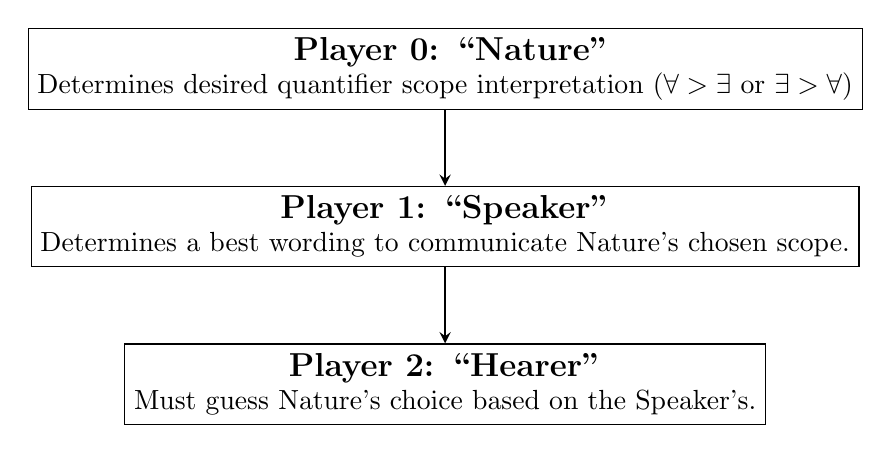
\begin{tikzpicture}[node distance=2cm]

	\node (nature) [box, align=center] {{\large \textbf{ Player 0: ``Nature''}}\\Determines desired quantifier scope interpretation (${\forall}>{\exists}$ or ${\exists}>{\forall}$)};
\node (speaker) [box, align=center, below of=nature] {{\large \textbf{Player 1: ``Speaker''}}\\Determines a best wording to communicate Nature's chosen scope. };
\node (hearer) [box, align=center, below of=speaker] {{\large \textbf{Player 2: ``Hearer''}}\\Must guess Nature's choice  based on the Speaker's.};

\draw [arrow] (nature) -- (speaker) ;
\draw [arrow] (speaker) -- (hearer) ;
\end{tikzpicture}
\end{center}
\end{figure}
\end{frame}





\section{Potential Solution}

\begin{frame}
\frametitle{Assumptions and Constraints}
\begin{itemize}\pause
\item It is generally preferable if quantifiers occur in the order they are supposed to be interpreted in (surface scope).\pause
\item Moving around nouns via `transformations' (passivization, clefting, etc.) is costly/marked/undesirable.\pause
\item Scrambling (to be discussed later), as opposed to transformations are not similarly costly.
\end{itemize}
\end{frame}


\begin{frame}
\frametitle{English Data}\pause
\begin{itemize}
\item Typical English sentences show scope ambiguity if there is more than one quantifier:\pause
\begin{exe}
\ex Two men dug each hole.
\end{exe}\pause
\item There can be two particular men who dig all the holes ($\exists>\forall$)  or, each hole can be dug by a different pair of men ($\forall>\exists$) .\pause
\item Ambiguity will usually disappear or become highly dispreferred if the sentence undergoes a `transformation:'\pause
\begin{exe}
\ex Each hole was dug by two men.
\end{exe}\pause
\item Here, the strongly preferred reading is the one where there is a pair of men for each hole ($\forall>\exists$), while the case where there is two specific men for each hole is harder to get out of the blue.
\end{itemize}
\end{frame}

\begin{frame}
\frametitle{English Data}\pause
\begin{exe}
\ex Everyone loves someone.\pause
\ex Everyone loves someone, and that person is Billy.\pause
\ex Everyone loves someone. Don't pretend like you don't have someone special.\pause
\ex Someone is loved by everyone.\pause
\ex Someone is loved by everyone, and that person is Billy.\pause
\ex[??]{ Someone is loved by everyone. Don't pretend like you don't have someone special.}
\end{exe}
\end{frame}

\begin{frame}
	\frametitle{Generalization in English}\pause

	\begin{itemize}
		\item Unmarked active sentences tend to be ambiguous.\pause
		\item Passive sentences tend to be unambiguous, preferring only surface scope.
	\end{itemize}

\end{frame}

\begin{frame}
	\frametitle{Now Onto the Game\ldots}\pause

	\begin{itemize}
		\item Both Players receive a payoff when the sentence is correctly communicated, represented by $x$.\pause
		\item If the more marked inverse scope is employed, both players suffer a slightly diminished payoff. We we refer to this amount as $i$.\pause
		\item If the Speaker employs passive voice, he suffers a slight loss $p$.\pause
		\item $|p+i|<|x|$ That is, even if we have to passivize and get inverse scope interpretation, it's always most preferable to get the intended interpretation.\pause
		\item This game is \textbf{non-zero sum Coordination Game}, meaning that both active players' interests are aligned.\pause
		\item The players \textbf{do not} have perfect information. While the Hearer knows what the Speaker's strategy is, he does not know what Nature has chosen.
	\end{itemize}

\end{frame}

\begin{frame}
\frametitle{The Decision Tree}
\begin{figure}
\footnotesize
\begin{forest} 
for tree={grow=east,draw=black,line width=0.2pt,parent anchor=east,child anchor=west,edge={draw=black},edge label={\Huge\color{black}},edge path={\noexpand\path[\forestoption{edge}](!u.parent anchor) -- ([xshift=-1.6cm].child anchor) --    
      (.child anchor)\forestoption{edge label};
  },
  l sep=2cm,
} 
[Nature,rectangle, s sep=25pt,
  [Speaker,edge label={node[Below]{$\exists>\forall$}}
    [Hearer,edge label={node[Below]{Passive}}
	[{$-p-i,-i$},edge label={node[Below]{Inverse}}]
	[{$x-p,x$},edge label={node[Below]{Surface}}]
	]
    [Hearer,edge label={node[Above]{Active}}
	[{$x-i,x-i$},edge label={node[Below]{Inverse}}]
	[{$0,0$},edge label={node[Below]{Surface}}]
	]
  ]
  [Speaker,edge label={node[Above]{$\forall>\exists$}}
    [Hearer,edge label={node[Below]{Passive}}
	[{$x-p-i,x-i$},edge label={node[Below]{Inverse}}]
	[{$-p,0$},edge label={node[Below]{Surface}}]
	]
    [Hearer,edge label={node[Above]{Active}}
	[{$-i,-i$},edge label={node[Below]{Inverse}}]
	[{$x,x$},edge label={node[Below]{Surface}}]
	]
  ]
]
\end{forest}
\caption{Decision Flow of the Game of ``Everybody loves somebody''}
\end{figure}
\end{frame}

\begin{frame}[fragile]
	\frametitle{Matrix for when Nature chooses $\forall > \exists$}
	\begin{center}
	\begin{figure}
	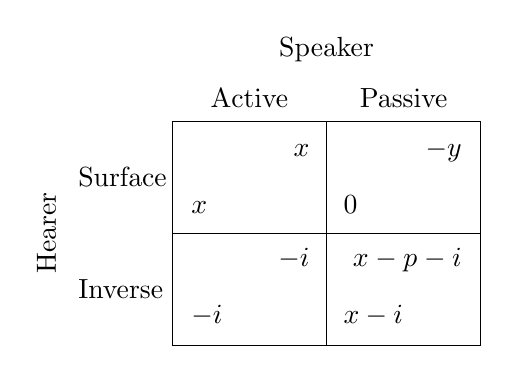
\begin{tikzpicture}
	\matrix[matrix of math nodes,every odd row/.style={align=right},every even row/.style={align=left},every node/.style={text width=1.5cm},row sep=0.2cm,column sep=0.2cm] (m) {
	$x$&$-y$\\
	$x$&$0$\\
	$-i$&$x-p-i$\\
	$-i$&$x-i$\\
	};
	\draw (m.north east) rectangle (m.south west);
	\draw (m.north) -- (m.south);
	\draw (m.east) -- (m.west);
	\coordinate (a) at ($(m.north west)!0.25!(m.north east)$);
	\coordinate (b) at ($(m.north west)!0.75!(m.north east)$);
	\node[above=5pt of a,anchor=base] {Active};
	\node[above=5pt of b,anchor=base] {Passive};
	\coordinate (c) at ($(m.north west)!0.25!(m.south west)$);
	\coordinate (d) at ($(m.north west)!0.75!(m.south west)$);
	\node[left=2pt of c,text width=1cm]  {Surface};
	\node[left=2pt of d,text width=1cm]  {Inverse};
	\node[above=18pt of m.north] (firm b) {Speaker};
	\node[left=1.6cm of m.west,rotate=90,align=center,anchor=center] {Hearer};
\end{tikzpicture}
	\caption{Decision Flow of the Game of ``Everybody loves somebody''}
\end{figure}
\end{center}
\end{frame}

\begin{frame}[fragile]
	\frametitle{Matrix for when Nature chooses $\exists > \forall$}
	\begin{center}
	\begin{figure}
	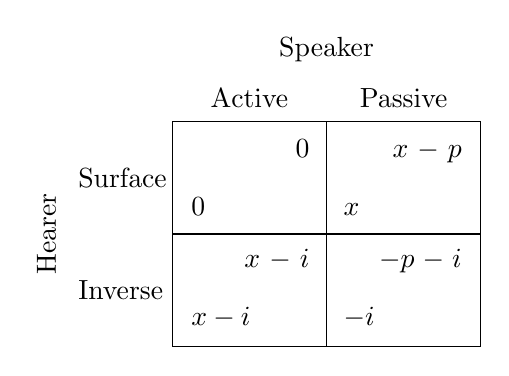
\begin{tikzpicture}
	\matrix[matrix of math nodes,every odd row/.style={align=right},every even row/.style={align=left},every node/.style={text width=1.5cm},row sep=0.2cm,column sep=0.2cm] (m) {
	$0$&$x-p$\\
	$0$&$x$\\
	$x-i$&$-p-i$\\
	$x-i$&$-i$\\
	};
	\draw (m.north east) rectangle (m.south west);
	\draw (m.north) -- (m.south);
	\draw (m.east) -- (m.west);
	\coordinate (a) at ($(m.north west)!0.25!(m.north east)$);
	\coordinate (b) at ($(m.north west)!0.75!(m.north east)$);
	\node[above=5pt of a,anchor=base] {Active};
	\node[above=5pt of b,anchor=base] {Passive};
	\coordinate (c) at ($(m.north west)!0.25!(m.south west)$);
	\coordinate (d) at ($(m.north west)!0.75!(m.south west)$);
	\node[left=2pt of c,text width=1cm]  {Surface};
	\node[left=2pt of d,text width=1cm]  {Inverse};
	\node[above=18pt of m.north] (firm b) {Speaker};
	\node[left=1.6cm of m.west,rotate=90,align=center,anchor=center] {Hearer};
	%\node[above=5pt of firm b]  {If Nature chooses $\forall>\exists$ in a scrambling language};
\end{tikzpicture}
	\caption{Decision Flow of the Game of ``Everybody loves somebody''}
\end{figure}
\end{center}
\end{frame}

\begin{frame}
	\frametitle{Results and Intuitive Explanation}\pause

	\begin{itemize}
		\item \textbf{Passivization is a kind of signalling.} If a speaker passivizes, which is costly, \emph{he does it for a reason}, probably to get a more preferable quantifier order.\pause
			\begin{itemize}
				\item This kind of signalling make the passive sentences \emph{unambiguous}.\pause
			\end{itemize}
		\item If the speaker \emph{does not} passivize, there are two options for the Hearer to choose from:\pause
			\begin{itemize}
				\item Either the active sentence is already in the right order\ldots\pause
				\item or it is not, but the Speaker didn't want to accrue the passive penalty ($p$).
			\end{itemize}
	\end{itemize}

\end{frame}

\begin{frame}
\frametitle{Scope in Scrambling Languages}\pause
\begin{itemize}
\item English has relatively rigid word order (subject-verb-object), but many languages have what is called `scrambling' which is free linear movement of nouns without the cost of transformations.\pause
\item Scope is systematically different in languages like these.\pause
\end{itemize}
\begin{exe}
\ex {\gll Har d\=aneshjui ye kit\=abi-ro mixune.\\
all student a book-OBJ reads\\
\trans{``Every student is reading a book.''}}\pause
\ex {\gll Ye ket\=abi-ro har d\=aneshjui mixune.\\
a book-OBJ all student reads\\
\trans{``Every student is reading a book.''}}
\end{exe}\pause
\begin{itemize}
\item However, both of these sentences \emph{must have} \textbf{surface scope}. They cannot be ambiguous.
\end{itemize}
\end{frame}

\begin{frame}
\frametitle{A Game Theoretic Account}\pause
\begin{itemize}
    \item Given our previous suggested constraints, we can predict these scope availabilities.\pause
    \item Remember, \textbf{surface scope} is preferred and \textbf{transformations} are costly.\pause
    \item However, \textbf{scrambling} is not similarly costly{\ldots} so it's a new strategy.
\end{itemize}
\end{frame}

\begin{frame}
\begin{figure}
\footnotesize
\begin{forest} 
for tree={grow=east,draw=black,line width=0.2pt,parent anchor=east,child anchor=west,edge={draw=black},edge label={\Huge\color{black}},edge path={\noexpand\path[\forestoption{edge}](!u.parent anchor) -- ([xshift=-1.6cm].child anchor) --    
      (.child anchor)\forestoption{edge label};
  },
  l sep=2cm,
} 
[Nature,rectangle, s sep=25pt,
  [Speaker,edge label={node[Below]{$\exists>\forall$}}
    [Hearer,edge label={node[Below]{Passive}}
	[{$-p-i,-p$},edge label={node[Below]{Inverse}}]
	[{$x-p,x$},edge label={node[Below]{Surface}}]
	]
    [Hearer,edge label={node[Above]{Active}}
	[{$x-i,x-i$},edge label={node[Below]{Inverse}}]
	[{$0,0$},edge label={node[Below]{Surface}}]
	]
[Hearer, edge label={node[Above]{Scramble}}
[{$-i,-i$}, edge label={node[Below]{Inverse}}]
[{$x,x$}, edge label={node[Below]{Surface}}]
]
  ]
  [Speaker,edge label={node[Above]{$\forall>\exists$}}
    [Hearer,edge label={node[Below]{Passive}}
	[{$x-p-i,x-i$},edge label={node[Below]{Inverse}}]
	[{$-p,0$},edge label={node[Below]{Surface}}]
	]
    [Hearer,edge label={node[Above]{Active}}
	[{$-i,-i$},edge label={node[Below]{Inverse}}]
	[{$x,x$},edge label={node[Below]{Surface}}]
	]
[Hearer, edge label={node[Above]{Scramble}}
[{$x-i,x-i$}, edge label={node[Below]{Inverse}}]
[{$0,0$}, edge label={node[Below]{Surface}}]
]
  ]
]
\end{forest}
\end{figure}
\end{frame}

	\begin{frame}
		\frametitle{Optimal Strategies with Scrambling}\pause

		\begin{itemize}
			\item First, Scramble is a \textbf{dominant strategy} over Passivization.\pause
			\item Since there is no longer cost to reordering for the Speaker, the focal strategies are to use whatever strategy avoids the need for inverse scope.\pause
			\item Seeing this, the Hearer's best strategy should always be to assume \textbf{surface scope}.\pause
			\item Therefore, for each sentence (active or scrambled), there should only be only one unambiguous interpretation.
		\end{itemize}

	\end{frame}

	\begin{frame}
		\frametitle{Formal Terms}\pause

		\begin{itemize}
			\item In all situations, we narrow down scope possibilies with \emph{Schelling Points}/focal points.\pause
			\item The ``markedness'' of inverted scope or passivization are \emph{vital} to communication, as they signal the Speaker's intention and indirectly create the focal points.
		\end{itemize}

	\end{frame}

\begin{frame}
\frametitle{In an English-like language\ldots}\pause
\begin{itemize}
\item As assumed speakers \emph{want} to interpret quantifiers in linear order.\pause
\item When a speaker produces a costly transformation (like a passive) the listener assumes that the new surface word order is the intended scope order.\pause
\item If a speaker produces an untransformed sentence, the listener has two possible hypotheses: (1) the speaker intended surface scope, or (2) that the speaker intended inverse scope, but didn't want to undergo a costly transformation.\pause
\item These two possibilities produce scope ambiguity.
\end{itemize}
\end{frame}


\begin{frame}
\frametitle{In Scrambling Languages}\pause
\begin{itemize}
\item In scrambling languages, since speakers have greater flexibility in ordering, listeners make different assumptions about intended scope.\pause
\item If the speaker wants the object to scope over the subject, he can easily scramble it leftward.\pause
\item Since he can do this, the unscrambled sentence has an unambiguous surface scope interpretation.\pause
\item \textbf{Sidenote:} Potentially related, languages with scrambling/flexible word order, usually rely on things like passivization less often.
\end{itemize}
\end{frame}


\begin{frame}
\frametitle{Just a random difference?}\pause
\begin{itemize}
\item In addition to this correlation between rigid word-order and scrambling languages, we see that this theory still hold in rigid constructions in scrambling languages.\pause
\item In Persian, for example, although nouns are flexible, negation must always be on the same part of a verb.\pause
\item We should expect negative quantifiers to work similar to English sentences in that they produce ambiguity. This is the case:\pause
\begin{exe}
\ex {\gll Billy ye ket\=abi-ro na-xund.\\
Billy a book-OBJ not-read\\
\trans{``Billy didn't read a (particular) book.'' ($\exists>\neg$)or ``Billy didn't read any book.'' ($\neg>\exists$)}}
\end{exe}\pause
\item This holds in similar languages with scrambling and stable negation location (e.g. Korean).

\end{itemize}
\end{frame}

\begin{frame}
	\frametitle{Rigidity = Ambiguity; Flexiblity = Unambiguousness}\pause

	\begin{itemize}
		\item The general theorem that arises from this analysis is that \emph{wherever} we have syntactic flexibility, we have ambiguity (and \textit{vice versa}.)\pause
		\item This difference, in agreement with our theory, is true \emph{across constructions}, not necessarily \emph{across languages}.\pause
		\item ``Scrambling'' languages are unambiguous in normal sentences, but are in more rigid constructions, ambiguity arises.\pause
			\begin{itemize}
				\item This is because the ambiguity is not a language-specific parameter, but a result of the strategies employable in any given context.
			\end{itemize}
	\end{itemize}

\end{frame}

\begin{frame}
	\frametitle{Local Rigidity}\pause
	In scrambling languages, generally we have syntactic flexibility accompanied by unambiguous surface scope.\pause
	
\begin{exe}
\ex \begin{xlist}\label{chin}
\ex[]{\gll Meigeren dou zhuazou yige {n\"uren}.\\
everyone all arrest a woman\\
	\trans{``Everyone arrested a woman.'' (${\forall}>{\exists} $)\label{chin1}}\pause
}
\ex[]{\gll (You) yige {n\"uren} meigeren dou zhuazou.\\
(have) a woman everyone all arrest.\\
	\trans{``A woman was arrested by everyone.'' (${\exists}>{\forall}$)\label{chin2}}
}\end{xlist}
\end{exe}\pause

But in syncactically inflexible constructions, ambiguity arises.\pause

\begin{exe}
\ex{ \begin{xlist}
\ex[]{\gll Meigeren dou bei yige {n\"uren} zhuazou.\\
everyone all PASS a woman arrest\\
	\trans{``Everyone was arrested by a woman.'' ($\forall > \exists$, ${\exists} > {\forall}$)\label{chin3}}\pause
}
\ex[*]{Bei yige {n\"uren} meigeren dou zhuazou.\\
PASS a woman everyone all arrest\\
\label{chin4}
}\end{xlist}}
\end{exe}
\end{frame}

\begin{frame}
	\frametitle{Local Rigidity in English as well}\pause

	English negation placement is \emph{rigid} with only one modal, as a result, the negation can take either wide or narrow scope.\pause

	\begin{exe}
		\ex Billy can not go. (${\forall}>{\exists}, {\exists}>{\forall}$)\pause
	\end{exe}

	On the other hand, where there are multiple modals, the negation can appear in multiple locations. This results in non-ambiguous sentences. (Note, the ambiguity is not with the \emph{could} modal, but \emph{have gone}.)\pause

	\begin{exe}
		\ex Billy could not have gone before we arrived.\label{could not}\pause
		\ex Billy could have not gone before we arrived.\label{have not}
	\end{exe}

\end{frame}

\begin{frame}
	\frametitle{But in languages where negation is \emph{always} flexible\ldots}

	{\ldots}like Chinese, we \emph{always} have a lack of ambiguity!

	\begin{exe}
		\ex {\gll Shujuan keyi \textbf{bu} gen Guorong {tiao wu}. \\
		Shujuan may not with Guorong dace \\
		\trans{``Shujuan is permitted not to dance with Guorong.'' ($may>{\neg}$)}}
		\ex {\gll Shujuan \textbf{bu} keyi gen Guorong {tiao wu}. \\
		Shujuan not may with Guorong dance \\
		\trans{``Shujuan can't dance with Guorong.'' (${\neg}>may$)}}
	\end{exe}

\end{frame}

\begin{frame}
	\frametitle{Empirical summary}\pause
	\centering

	\begin{tabular}{l|l}
		Rigid constructions & Flexible constructions\\\hline\pause
		English main clauses&Main clauses in scrambling languages\\\pause
		Persian negation&Chinese negation\\\pause
		English negation with auxes&English negation without auxes\\\pause
		Chinese passives&English Passives*\\\pause
		\textbf{All of these are ambiguous.}&\textbf{All of these are non-ambiguous.}
	\end{tabular}
\end{frame}

\begin{frame}
	\frametitle{The General Theory}\pause

	\begin{itemize}
		\item Quantifier scope interpretaions are not so much syntactically \emph{licensed} so much as they are \textbf{pruned} from the all possible combinations of scopes ($q!$ where $q=$ number of quantifiers).\pause
			\begin{itemize}
				\item That is, \emph{all} quantifier scope interpretations are possible in the abstract (hence Chomsky's aphasia)\ldots\pause
				\item but the pragmatics of the structure of a language (what other constructions we have available) determine what are actually plausible interpretations.\pause
			\end{itemize}

		\item Without any syntactic machinery, we have already done a lot of the work of narrowing in on what interpretations are possible.\pause
		\item But the story is not done yet!
	\end{itemize}
\end{frame}

\begin{frame}
\frametitle{Project Extension}\pause
	\begin{itemize}
		\item Replace generative notions of syntactically-determined quantifier scope ambiguities with more plausible, externally-driven factors.\pause
		\item Unify this account with other scope alternations (say, the unavailability of semantically implausible scope interpretations) into a general theory of scope where possible interpretations are \emph{pruned}, rather than derived by some syntactic engine.\pause
		\item Similar accounts for related phenomena? C-command? Cross-over?
		\item Extensive Game Theory w.r.t different quantifiers and remodelling given data.
	\end{itemize}
\end{frame}

\begin{frame}
	\frametitle{The End}
	\begin{center}
	%\includegraphics[height=.85\textheight]{toon.png}
\end{center}

\end{frame}

\end{document}
